\documentclass[12pt, twoside]{book}
%\documentclass[12pt, oneside]{book}  % jednostranna tlac
\usepackage[a4paper,top=2.5cm,bottom=2.5cm,left=3.5cm,right=2cm]{geometry}
\usepackage[utf8]{inputenc}
\usepackage[T1]{fontenc}
\usepackage{graphicx}
\usepackage{url}
\usepackage[hidelinks,breaklinks]{hyperref}
\usepackage[slovak]{babel} % vypnite pre prace v anglictine
\usepackage{float}
% https://tex.stackexchange.com/questions/37581/latex-figures-side-by-side
\usepackage{subcaption} % obrazky vedla seba
\linespread{1.25} % hodnota 1.25 by mala zodpovedat 1.5 riadkovaniu

% -------------------
% --- Definicia zakladnych pojmov
% --- Vyplnte podla vasho zadania
% -------------------
\def\mfrok{2018}
\def\mfnazov{Učebné prostredie pre online kolektívny vývoj agilných programov za pomoci zdieľateľného editoru}
\def\mftyp{Bakalárska práca}
\def\mfautor{Emanuel Tesař}
\def\mfskolitel{Ing. František Gyarfaš, CSc.}

%ak mate konzultanta, odkomentujte aj jeho meno na titulnom liste
%\def\mfkonzultant{tit. Meno Priezvisko, tit. }  

\def\mfmiesto{Bratislava, \mfrok}

% bioinformatici odkomentujú riadok s dvoma odbormi
\def\mfodbor{ Informatika}
%\def\mfodbor{ Informatika a Biológia } 
\def\program{ Informatika }
% Ak je školiteľ z FMFI, uvádzate katedru školiteľa, zrejme by mala byť aj na zadaní z AIS2
% Ak máte externého školiteľa, uvádzajte Katedru informatiky 
\def\mfpracovisko{ Katedra aplikovanej informatiky }

\begin{document}     
\frontmatter


% -------------------
% --- Obalka ------
% -------------------
\thispagestyle{empty}

\begin{center}
\sc\large
Univerzita Komenského v Bratislave\\
Fakulta matematiky, fyziky a informatiky

\vfill

{\LARGE\mfnazov}\\
\mftyp
\end{center}

\vfill

{\sc\large 
\noindent \mfrok\\
\mfautor
}

\cleardoublepage
% --- koniec obalky ----

% -------------------
% --- Titulný list
% -------------------

\thispagestyle{empty}
\noindent

\begin{center}
\sc  
\large
Univerzita Komenského v Bratislave\\
Fakulta matematiky, fyziky a informatiky

\vfill

{\LARGE\mfnazov}\\
\mftyp
\end{center}

\vfill

\noindent
\begin{tabular}{ll}
Študijný program: & \program \\
Študijný odbor: & \mfodbor \\
Školiace pracovisko: & \mfpracovisko \\
Školiteľ: & \mfskolitel \\
% Konzultant: & \mfkonzultant \\
\end{tabular}

\vfill


\noindent \mfmiesto\\
\mfautor

\cleardoublepage
% --- Koniec titulnej strany


% -------------------
% --- Zadanie z AIS
% -------------------
% v tlačenej verzii s podpismi zainteresovaných osôb.
% v elektronickej verzii sa zverejňuje zadanie bez podpisov
% v pracach v naglictine anglicke aj slovenske zadanie

\newpage 
\thispagestyle{empty}
\hspace{-2cm}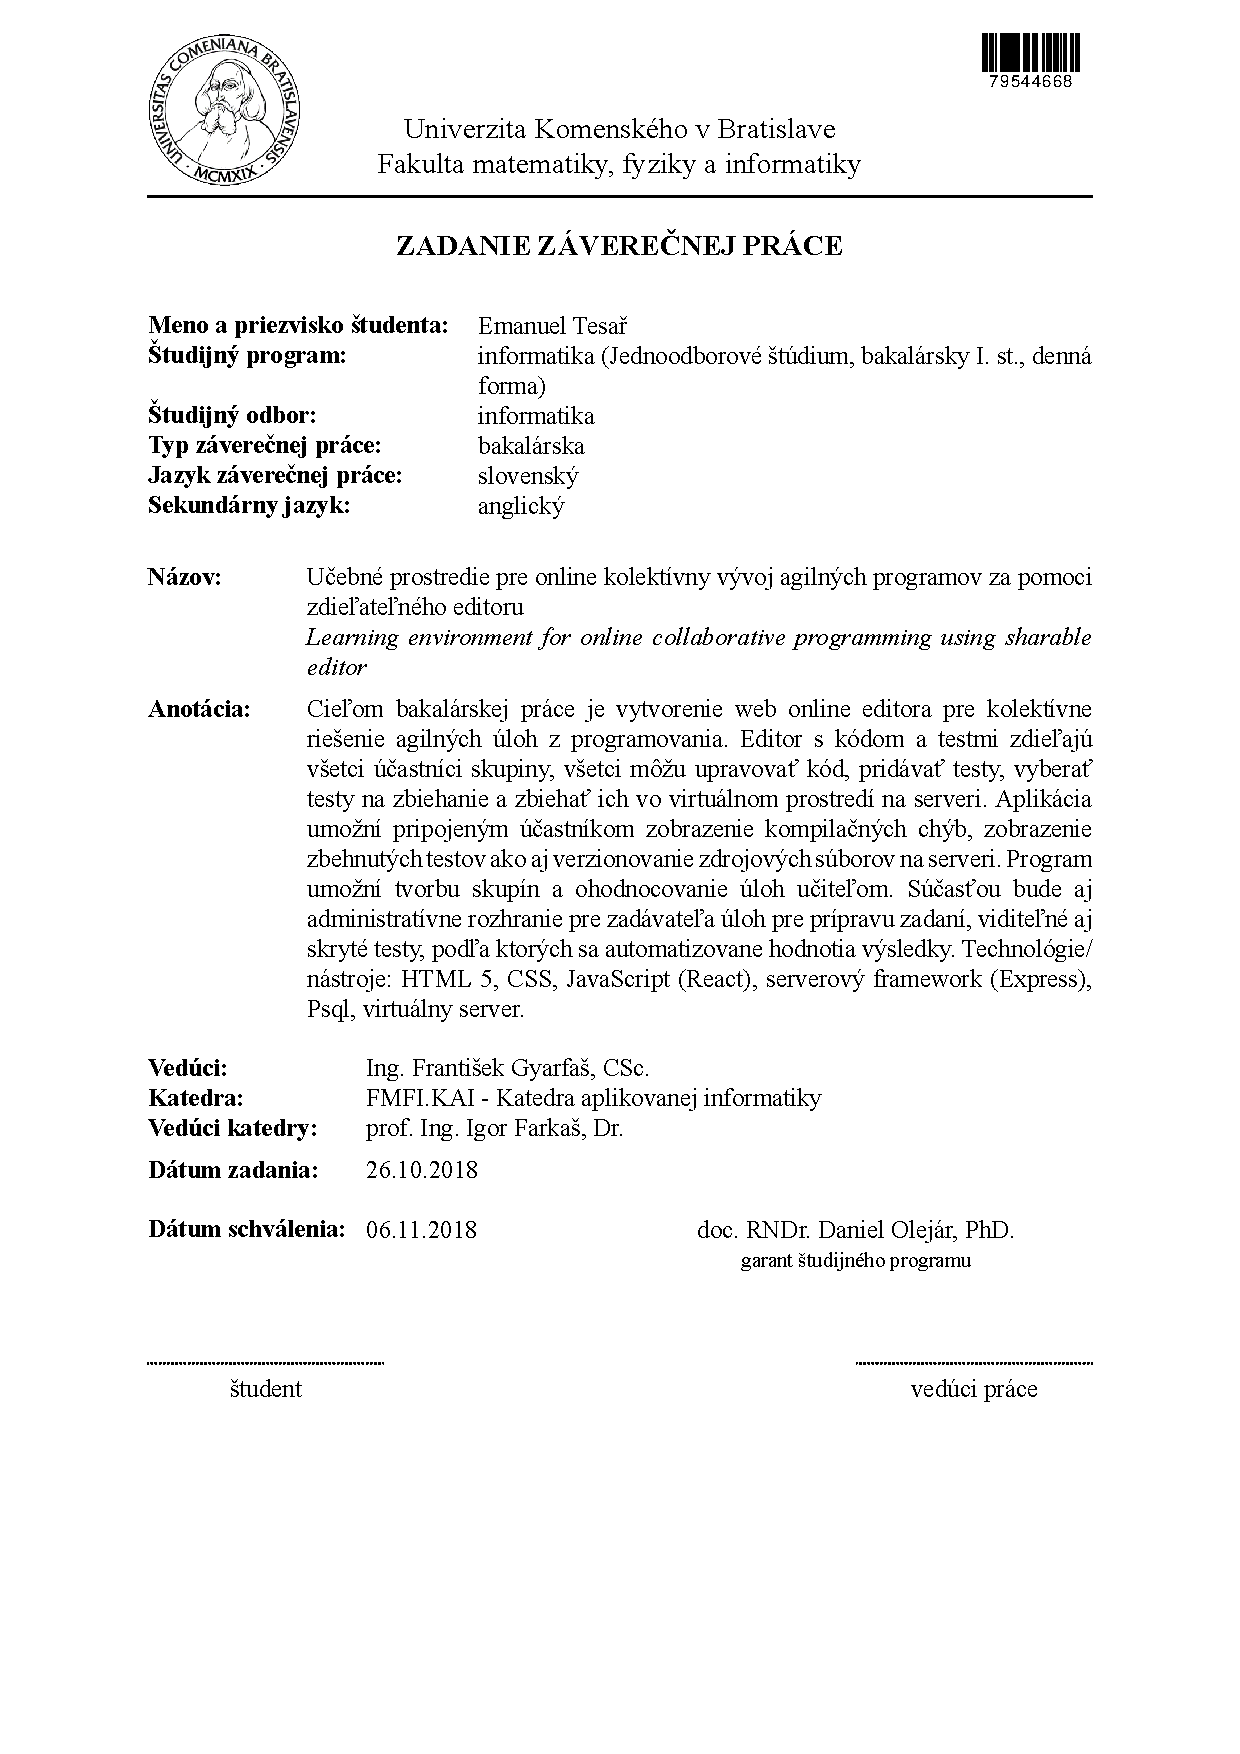
\includegraphics[width=1.1\textwidth]{images/zadanie}

% --- Koniec zadania

\frontmatter

% -------------------
%   Poďakovanie - nepovinné
% -------------------
\setcounter{page}{3}
\newpage 
~

\vfill
{\bf Poďakovanie:} Ďakujem môjmu školiteľovi Ing. Františkovi Gyarfašovi, CSc. za užitočné 
pripomienky, ochotu a usmernenie pri písaní diplomovej práce. Taktiež ďakujem svojej rodine 
a frejerke za ich pomoc a motiváciu.
% --- Koniec poďakovania

% -------------------
%   Abstrakt - Slovensky
% -------------------
\newpage 
\section*{Abstrakt}
Cieľom práce bol návrh a funkčná implementácia zdieľateľného editora podporujúca
súbežné písanie kódu viacerých používateľov. Používatelia okrem písania kódu, môžu pridávať
testy, ktoré sa dajú spustiť vo virtuálnom prostredí na serveri. V prípade neskompilovateľného kódu, 
chyby počas behu programu, prípadne inej chyby, zobrazí chybovú hlášku. Okrem pohodlného prostredia
pre používateľa obsahuje aj administrátorské rozhranie, v ktorom sa dajú pridávať neviditeľné testy 
pre používateľov. Toto rozhranie umožňuje profesorom vytvárať zadania pre
študentov, ktorí následne môžu úlohu riešiť priamo vo webovom prehliadači.

\paragraph*{Kľúčové slová:} CRDT, kolaboratívne upravovanie, synchronizácia
% --- Koniec Abstrakt - Slovensky


% -------------------
% --- Abstrakt - Anglicky 
% -------------------
\newpage 
\section*{Abstract}
The aim of the work was to design and implement a shared editor supporting
collaborative editing of multiple users. In addition to writing code, users can add
tests that can run in a virtual server environment. In the case of uncompressed code,
errors during program run, or other errors, will display an error message. 
In addition to a comfortable environment it also has an administrative interface
for the user to add invisible tests for users. This interface allows professors to create
assignments for students who can then solve the task directly in the web browser.

\paragraph*{Keywords:} CRDT, collaborative editing, synchronization


% --- Koniec Abstrakt - Anglicky

% -------------------
% --- Predhovor - v informatike sa zvacsa nepouziva
% -------------------
%\newpage 
%\thispagestyle{empty}
%
%\huge{Predhovor}
%\normalsize
%\newline
%Predhovor je všeobecná informácia o práci, obsahuje hlavnú charakteristiku práce 
%a okolnosti jej vzniku. Autor zdôvodní výber témy, stručne informuje o cieľoch 
%a význame práce, spomenie domáci a zahraničný kontext, komu je práca určená, 
%použité metódy, stav poznania; autor stručne charakterizuje svoj prístup a svoje 
%hľadisko. 
%
% --- Koniec Predhovor


% -------------------
% --- Obsah
% -------------------

\newpage 

\tableofcontents

% ---  Koniec Obsahu

% -------------------
% --- Zoznamy tabuliek, obrázkov - nepovinne
% -------------------

\newpage 

\listoffigures
\listoftables

% ---  Koniec Zoznamov

\mainmatter


\input uvod.tex 

\input kapitola1.tex

\input kapitola2.tex

\input kapitola3.tex

\input kapitola4.tex

\input kapitola5.tex

\input kapitola6.tex

\input zaver.tex

% -------------------
% --- Bibliografia
% -------------------


\newpage	

\backmatter

\thispagestyle{empty}
\nocite{*}
\clearpage

\bibliographystyle{plain}
\bibliography{literatura} 

%Prípadne môžete napísať literatúru priamo tu
%\begin{thebibliography}{5}
 
%\bibitem{br1} MOLINA H. G. - ULLMAN J. D. - WIDOM J., 2002, Database Systems, Upper Saddle River : Prentice-Hall, 2002, 1119 s., Pearson International edition, 0-13-098043-9

%\bibitem{br2} MOLINA H. G. - ULLMAN J. D. - WIDOM J., 2000 , Databasse System implementation, New Jersey : Prentice-Hall, 2000, 653s., ???

%\bibitem{br3} ULLMAN J. D. - WIDOM J., 1997, A First Course in Database Systems, New Jersey : Prentice-Hall, 1997, 470s., 

%\bibitem{br4} PREFUSE, 2007, The Prefuse visualization toolkit,  [online] Dostupné na internete: <http://prefuse.org/>

%\bibitem{br5} PREFUSE Forum, Sourceforge - Prefuse Forum,  [online] Dostupné na internete: <http://sourceforge.net/projects/prefuse/>

%\end{thebibliography}

%---koniec Referencii

% -------------------
%--- Prilohy---
% -------------------

%Nepovinná časť prílohy obsahuje materiály, ktoré neboli zaradené priamo  do textu. Každá príloha sa začína na novej strane.
%Zoznam príloh je súčasťou obsahu.
%
%\addcontentsline{toc}{chapter}{Appendix A}
%\input AppendixA.tex
%
%\addcontentsline{toc}{chapter}{Appendix B}
%\input AppendixB.tex

\end{document}
